%%%%%%%%%%%%%%%%%%%%%%%%%%%%%%%%%%%%%%%%%
% Structured General Purpose Assignment
% LaTeX Template
%
% This template has been downloaded from:
% http://www.latextemplates.com
%
% Original author:
% Ted Pavlic (http://www.tedpavlic.com)
%
% Note:
% The \lipsum[#] commands throughout this template generate dummy text
% to fill the template out. These commands should all be removed when 
% writing assignment content.
%
%%%%%%%%%%%%%%%%%%%%%%%%%%%%%%%%%%%%%%%%%

%----------------------------------------------------------------------------------------
%	PACKAGES AND OTHER DOCUMENT CONFIGURATIONS
%----------------------------------------------------------------------------------------

\documentclass{article}

\usepackage{fancyhdr} % Required for custom headers
\usepackage{lastpage} % Required to determine the last page for the footer
\usepackage{extramarks} % Required for headers and footers
\usepackage{graphicx} % Required to insert images
\usepackage{lipsum} % Used for inserting dummy 'Lorem ipsum' text into the template
\usepackage{amsmath}
\usepackage{hyperref}

% Margins
\topmargin=-0.45in
\evensidemargin=0in
\oddsidemargin=0in
\textwidth=6.5in
\textheight=9.0in
\headsep=0.25in 

\linespread{1.1} % Line spacing

% Set up the header and footer
\pagestyle{fancy}
\lhead{\hmwkAuthorName} % Top left header
\chead{\hmwkClass\ (\hmwkClassInstructor\ \hmwkClassTime): \hmwkTitle} % Top center header
\rhead{\firstxmark} % Top right header
\lfoot{\lastxmark} % Bottom left footer
\cfoot{} % Bottom center footer
\rfoot{Page\ \thepage\ of\ \pageref{LastPage}} % Bottom right footer
\renewcommand\headrulewidth{0.4pt} % Size of the header rule
\renewcommand\footrulewidth{0.4pt} % Size of the footer rule

\setlength\parindent{0pt} % Removes all indentation from paragraphs

%----------------------------------------------------------------------------------------
%	DOCUMENT STRUCTURE COMMANDS
%	Skip this unless you know what you're doing
%----------------------------------------------------------------------------------------

% Header and footer for when a page split occurs within a problem environment
\newcommand{\enterProblemHeader}[1]{
\nobreak\extramarks{#1}{#1 continued on next page\ldots}\nobreak
\nobreak\extramarks{#1 (continued)}{#1 continued on next page\ldots}\nobreak
}

% Header and footer for when a page split occurs between problem environments
\newcommand{\exitProblemHeader}[1]{
\nobreak\extramarks{#1 (continued)}{#1 continued on next page\ldots}\nobreak
\nobreak\extramarks{#1}{}\nobreak
}

\setcounter{secnumdepth}{0} % Removes default section numbers
\newcounter{homeworkProblemCounter} % Creates a counter to keep track of the number of problems

\newcommand{\homeworkProblemName}{}
\newenvironment{homeworkProblem}[1][Problem \arabic{homeworkProblemCounter}]{ % Makes a new environment called homeworkProblem which takes 1 argument (custom name) but the default is "Problem #"
\stepcounter{homeworkProblemCounter} % Increase counter for number of problems
\renewcommand{\homeworkProblemName}{#1} % Assign \homeworkProblemName the name of the problem
\section{\homeworkProblemName} % Make a section in the document with the custom problem count
\enterProblemHeader{\homeworkProblemName} % Header and footer within the environment
}{
\exitProblemHeader{\homeworkProblemName} % Header and footer after the environment
}

\newcommand{\problemAnswer}[1]{ % Defines the problem answer command with the content as the only argument
\noindent\framebox[\columnwidth][c]{\begin{minipage}{0.98\columnwidth}#1\end{minipage}} % Makes the box around the problem answer and puts the content inside
}

\newcommand{\homeworkSectionName}{}
\newenvironment{homeworkSection}[1]{ % New environment for sections within homework problems, takes 1 argument - the name of the section
\renewcommand{\homeworkSectionName}{#1} % Assign \homeworkSectionName to the name of the section from the environment argument
\subsection{\homeworkSectionName} % Make a subsection with the custom name of the subsection
\enterProblemHeader{\homeworkProblemName\ [\homeworkSectionName]} % Header and footer within the environment
}{
\enterProblemHeader{\homeworkProblemName} % Header and footer after the environment
}
   
%----------------------------------------------------------------------------------------
%	NAME AND CLASS SECTION
%----------------------------------------------------------------------------------------

\newcommand{\hmwkTitle}{Midterm} % Assignment title
\newcommand{\hmwkDueDate}{Tuesday,\ August\ 29,\ 2017} % Due date
\newcommand{\hmwkClass}{ANLY\ 515-50-2017} % Course/class
\newcommand{\hmwkClassTime}{} % Class/lecture time
\newcommand{\hmwkClassInstructor}{Dr. Martin A. Negron} % Teacher/lecturer
\newcommand{\hmwkAuthorName}{Nelson Corrocher} % Your name

%----------------------------------------------------------------------------------------
%	TITLE PAGE
%----------------------------------------------------------------------------------------

\title{
\vspace{2in}
\textmd{\textbf{\hmwkClass:\ \hmwkTitle}}\\
\normalsize\vspace{0.1in}\small{Due\ on\ \hmwkDueDate}\\
\vspace{0.1in}\large{\textit{\hmwkClassInstructor\ \hmwkClassTime}}
\vspace{3in}
}

\author{\textbf{\hmwkAuthorName}}
\date{Friday,\ August\ 25,\ 2017} % Insert date here if you want it to appear below your name

%----------------------------------------------------------------------------------------

\begin{document}

\maketitle

%----------------------------------------------------------------------------------------
%	TABLE OF CONTENTS
%----------------------------------------------------------------------------------------

%\setcounter{tocdepth}{1} % Uncomment this line if you don't want subsections listed in the ToC

\newpage
\tableofcontents
\newpage

%----------------------------------------------------------------------------------------
%	PROBLEM 1
%----------------------------------------------------------------------------------------

\begin{homeworkProblem}[Problem \#\arabic{homeworkProblemCounter}] % Custom section title
The US Federal Motor Carrier Safety Administration planned in 2013 to issue rules that would limit the number of hours per week that truck drivers can work. The rules would reduce driver workweeks (fewer hours), restrict the number of nights that truckers can work, and require rest breaks during the day. The impacts could include keeping sleep deprived drivers off the road, reducing crashes, preventing fatigue-related crashes, improving working conditions, reducing driver turnover, improving driver safety, saving lives, reducing injuries, and reducing fatigue-related health problems.
	
	%--------------------------------------------
	
	\begin{homeworkSection}{(a)} % Section within problem
		Identify 3 risks associated with this information
		
		\problemAnswer{ % Answer
			\begin{itemize}
				\item To compensate for less hours and lower salary, drivers could start a second job, decreasing some of the benefits like fatigue-related health problems and crashes.
				\item To compensate for less hours and lower salary, drivers may try to drive faster, which would decrease safety and increase crashes.
				\item To compensate for less hours and lower salary, drivers may overload the truck to carry more cargo, decreasing safety and increasing crashes.
			\end{itemize}
		}
		
	\end{homeworkSection}
	
	%--------------------------------------------
	
	\begin{homeworkSection}{(b)} % Section within problem
		 Using  the  risk/opportunity  approach,  develop  a  conceptual  model  including events, triggers, mitigation, control and consequences
		
		\problemAnswer{ % Answer
			\begin{center}
				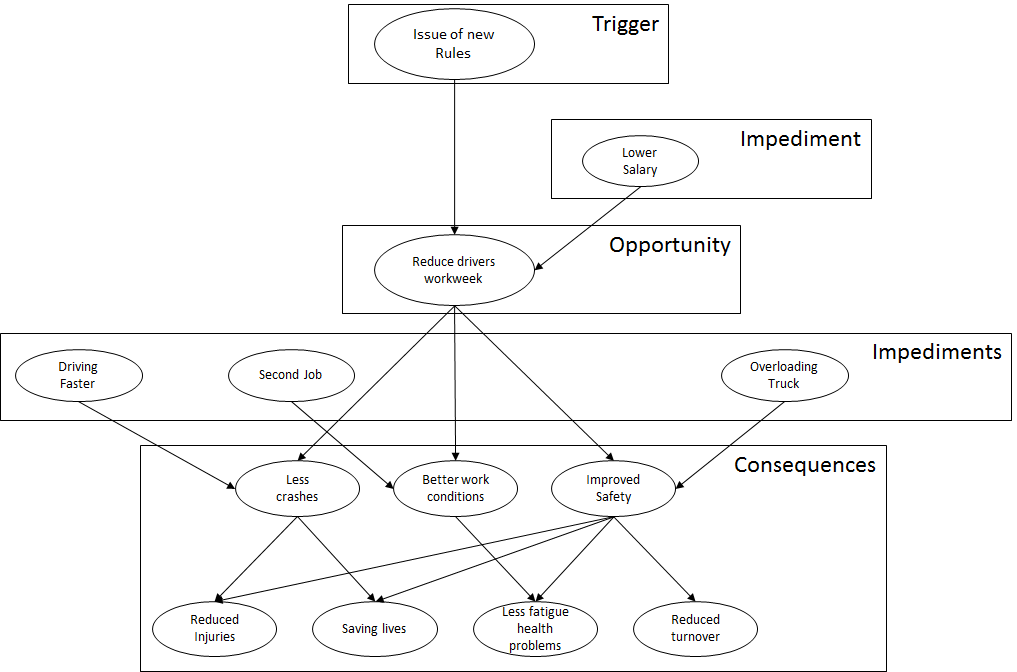
\includegraphics[width=\textwidth,keepaspectratio]{1b.png} % Example image
			\end{center}
		}
		
	\end{homeworkSection}
	
	%--------------------------------------------
	
\end{homeworkProblem}

%----------------------------------------------------------------------------------------
%	PROBLEM 2
%----------------------------------------------------------------------------------------

\begin{homeworkProblem}[Problem \#\arabic{homeworkProblemCounter}] % Custom section title
There are three identical and independent temperature sensors that will trigger in:
\begin{itemize}
	\item 90\% of the cases where the temperature is high.
	\item 5\% of the cases where the temperature is nominal.
	\item 1\% of the cases where the temperature is low.
\end{itemize}



\begin{center}
	\begin{tabular}{||c c c c||} 
		\hline
		(T)emperature & L & N & H \\ [0.5ex] 
		\hline\hline
		True & 0.01 & 0.05 & 0.9 \\ 
		\hline
		False & 0.99 & 0.95 & 0.1 \\
		\hline
	\end{tabular}
\end{center}

The probability of high temperature is 20\%, nominal temperature is 70\%, and low temperature is 10\%. Describe a Bayesian network and corresponding queries for computing the following:

\begin{center}
	\begin{tabular}{||c c c||} 
		\hline
		(T)emperature & True & False \\ [0.5ex] 
		\hline\hline
		H & 0.2 & 0.8 \\ 
		\hline
		N & 0.7 & 0.3 \\
		\hline
		L & 0.1 & 0.9 \\
		\hline
	\end{tabular}
\end{center}

Below the tabular version for calculating the marginal probabilities of the Sensors

\begin{center}
	\begin{tabular}{||c c c c c||} 
		\hline
		& H & N & L & P(S) \\ [0.5ex] 
		\hline\hline
		True & 0.18 & 0.035 & 0.001 & 0.216 \\ 
		\hline
		False & 0.02 & 0.665 & 0.099 & 0.784 \\
		\hline
		P(T) & 0.2 & 0.7 & 0.1 & 1 \\
		\hline
				
	\end{tabular}
\end{center}

The Bayes networks equations to calculate the probabilities can be long and error prone when done manually. Since the book and slides recommends using AgenaRisk for representations and calculations, this is method I decided to use here.

%--------------------------------------------

\clearpage
\begin{homeworkSection}{(a)} % Section within problem
Probability that the first sensor will trigger given that the other two sensors have also triggered.

\problemAnswer{ % Answer
	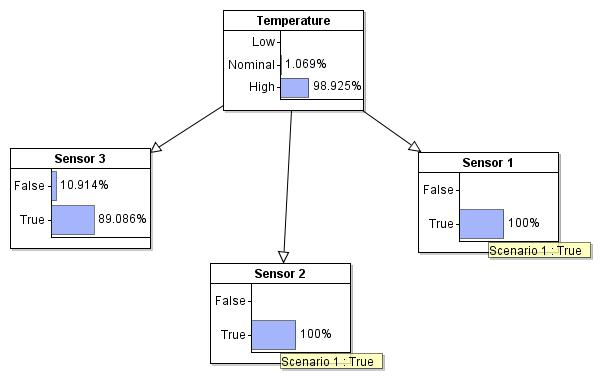
\includegraphics[width=\textwidth,keepaspectratio]{3a.jpg}\\
	Thus, the probability is \textbf{89.1\%}
	
	
}
\end{homeworkSection}

%--------------------------------------------
\clearpage
\begin{homeworkSection}{(b)} % Section within problem
Probability that the temperature is high given that all three sensors have triggered.

\problemAnswer{ % Answer
	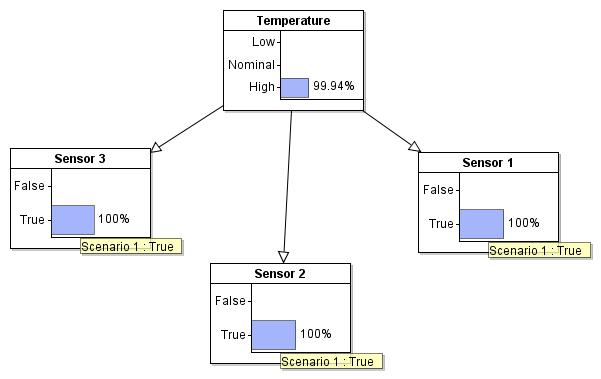
\includegraphics[width=\textwidth,keepaspectratio]{3b.jpg}\\
		Thus, the probability is \textbf{99.94\%}
}
\end{homeworkSection}

%--------------------------------------------
\clearpage
\begin{homeworkSection}{(c)} % Section within problem
Probability that the temperature is high given that at least one sensor has triggered.

	\problemAnswer{ % Answer
		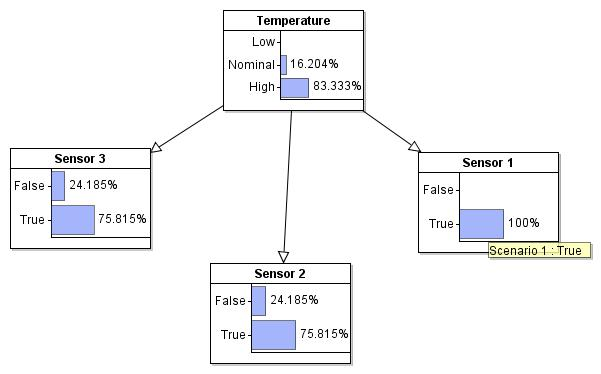
\includegraphics[width=\textwidth,keepaspectratio]{3c.jpg}\\
		Thus, the probability is \textbf{83.33\%}
	}
\end{homeworkSection}

%--------------------------------------------

\end{homeworkProblem}

\clearpage
%----------------------------------------------------------------------------------------
%	PROBLEM 3
%----------------------------------------------------------------------------------------

\begin{homeworkProblem}[Problem \#\arabic{homeworkProblemCounter}] % Roman numerals
A few weeks after inseminating a cow, we have three possible tests to confirm pregnancy. The first is a scanning test (S) that has a false positive of 1\% and a false negative of 10\%. The second is a blood test (B) that detects progesterone with a false positive of 10\% and a false negative of 30\%. The third test is a urine test (U) that also detects progesterone with a false positive of 10\% and a false negative of 20\%. The probability of a detectable progesterone level is 90\% given pregnancy and 1\% given no pregnancy. The probability that insemination will impregnate a cow is 87\%. Suppose now that we inseminate a cow, wait for a few weeks, and then perform the three tests, which all come out negative. Using a Bayesian model determine the probability that the cow is pregnant?\\\\

%--------------------------------------------

\problemAnswer{ % Answer
	The model for the exercise was designed using AgenaRisk and is shown in the image below.\\\\
	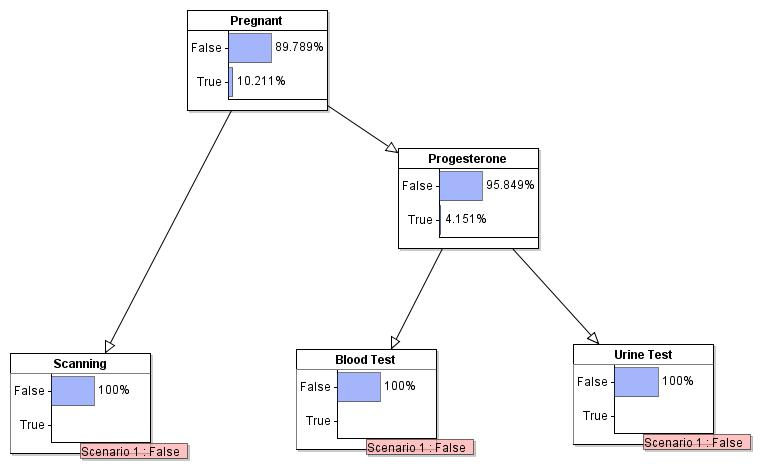
\includegraphics[width=\textwidth,keepaspectratio]{3.jpg}\\
	Thus, the probability of the cow being pregnant after the three tests returned negative is \textbf{10.21\%}
}

\end{homeworkProblem}
\clearpage
%----------------------------------------------------------------------------------------
%	PROBLEM 4
%----------------------------------------------------------------------------------------

\begin{homeworkProblem}[Problem \#\arabic{homeworkProblemCounter}] % Roman numerals
	A manufacturing firm has signed a contract to produce a product to demand, receiving \$500 per unit. The firm could either produce the product itself or outsource the production. Demand is exponentially distributed with a mean of 10,000 units per year. In-house production has normally-distributed fixed costs with mean of \$500,000 and a standard deviation of \$100,000 and normally-distributed variable costs with mean \$200 and standard deviation of \$10. Outsourcing has no fixed cost, but variable costs are \$250.

	\begin{homeworkSection}{(a)} % Section within problem
	Create a diagram for this problem.
	
	\problemAnswer{
		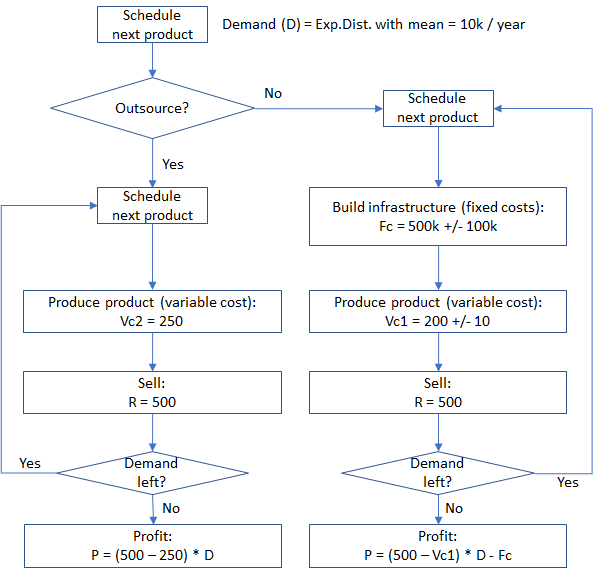
\includegraphics[width=\textwidth,keepaspectratio]{4a.png} % Example image % Answer
	}
	
	\end{homeworkSection}

%--------------------------------------------

	\clearpage
	\begin{homeworkSection}{(b)} % Section within problem
	Forecast the profit for each alternative.
	
	\problemAnswer{ % Answer
		Analytically, we have two models: Producing in-house (Model 1) and outsourcing (Model 2). Calculating the profit for each of the equations from (a).\\
		Model 1: \\
		\begin{equation*}
		\begin{split}
		P1 	&= (Revenue - Cost) * D - FC1\\
			&= (500 - VC1) * D - FC1 \\
			&= (500 - 200) * 10000 - 500000 \\
			&= 2,500,000
		\end{split}
		\end{equation*}
		\\
		Model 2: \\
		\begin{equation*}
		\begin{split}
		P2 	&= (Revenue - Cost) * D \\
			&= (500 - 250) * 10000 \\
			&= 2,500,000
		\end{split}
		\end{equation*}
		\\
		
	}
	
	\end{homeworkSection}

%--------------------------------------------

\begin{homeworkSection}{(c)} % Section within problem
	Determine the difference in profit.
	
	\problemAnswer{ % Answer
		Analytically speaking, on average, the profit for both models is the same and thus, the difference between them is zero.
		For demand(D) less lower than 10,000, outsourcing (Model 2) provides greater profits and above the 10,000 it becomes more profitable to produce in-house. \\
	}
	
\end{homeworkSection}

	%--------------------------------------------
	\clearpage
	\begin{homeworkSection}{(d)} % Section within problem
	Determine the probability that each alternative achieves at least \$0, \$100,000 and \$200,000 profit.
		
		\problemAnswer{ % Answer
			For Model 2, the probability can be calculated by solving the equation for demand when the profits are \$0, \$100,000 and \$200,000. The demand (D) required for these values is, respectively, 0, 200 and 400. This can be easily calculate by getting the cumulative probability of these values in a exponential distribution. In Excel, this is simply done by using \textbf{= 1 - EXPON.DIST('D',1/10000,1)} with D being equal to the values above.
			Using the exponential distribution, we get the probabilities of 100\%, 98.02\% and 96.08\%. \\
			\\
			For Model 1, the calculation become more complicated because the probability distribution now is a combination of two normal distributions, one for each cost, and an exponential distribution, for the demand. The approach used to calculate this distribution is to use Monte Carlo simulation in Excel (MCSim addin, available at \url{http://www3.wabash.edu/econometrics/EconometricsBook/Basic\%20Tools/ExcelAddIns/MCSim.htm}).\\\\
			Assuming a confidence interval of 95\%:\\\\
			For profit \textgreater= 0, P(profit \textgreater= 0) = 84.80 +/- 0.22\% \\
			For profit \textgreater= 100,000, P(profit \textgreater= 100,000) = 81.77 +/- 0.24\% \\
			For profit \textgreater= 200,000, P(profit \textgreater= 200,000) = 79.41 +/- 0.25\% \\\\
			One important note is that in opposite of Model 2, the profit in Model 1 will be negative (loss) in about 15\% of the time.
		}
		
	\end{homeworkSection}

\end{homeworkProblem}

%----------------------------------------------------------------------------------------

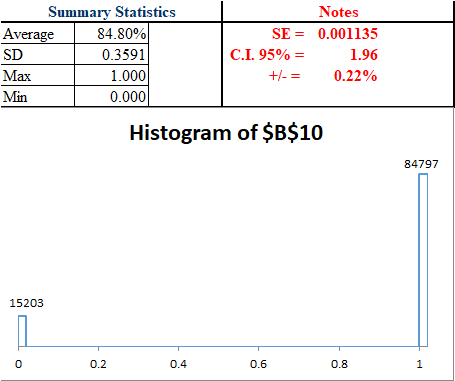
\includegraphics[width=\textwidth,keepaspectratio]{4d1.png}
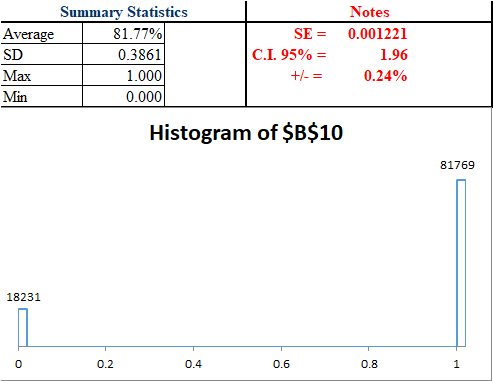
\includegraphics[width=\textwidth,keepaspectratio]{4d2.png}
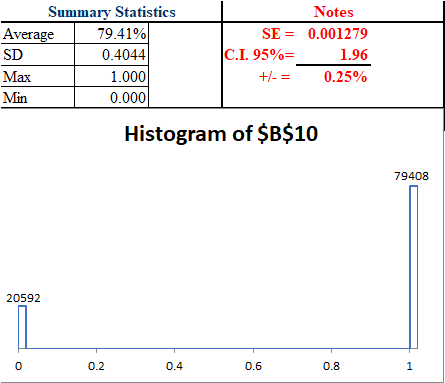
\includegraphics[width=\textwidth,keepaspectratio]{4d3.png}

\end{document}
